\chapter{Results}\label{chp.results}
In this chapter, the results are summarized and analyzed. 
In Section~\ref{sec.results.overview},
some descriptive statistics are provided, and 
the Stroop effects on different experiment groups from 
Table~\ref{tab.hypothesis.whole.design} are examined;
in addition,
the hypothesizes described in Section~\ref{sec.hypothesis} are tested per items in Section~\ref{sec.results.hypothesis}.



\section{Overview}\label{sec.results.overview}
\begin{table}[!b]
\centering
\ra{1.7}
\caption{Overall statistics for accuracy rate and response time. In addition,
the two-tailed p-value from a paired t-test is also reported.}\label{tab.results.overview}
\resizebox{0.7\textwidth}{!}{
\begin{tabular}{@{}cccc@{}}
\toprule
		& mean (congruent) & mean (incongruent) & p-value \\
   \midrule
accuracy&$0.89$&$0.83$&$p < 0.001$\\
response time&$503.2$~ms&$537.8$~ms&$p < 0.001$\\
\bottomrule
\end{tabular}
}
\end{table}



\begin{table}[!t]
\centering
\ra{1.7}
\caption{The accuracy rate with (SD) for the production of facial expressions in the different conditions.}
\label{tab.results.accuracyrate}
\resizebox{0.7\textwidth}{!}{
\begin{tabular}{@{}ccc|cc@{}}
\toprule
\multicolumn{3}{c|}{experiment conditions}& adults' faces &babies' faces\\
\midrule
\multirow{4}{*}{mother}&\multirow{2}{*}{positive}&``Freude''&$0.91(0.06)$&$0.91(0.08)$\\
&&``Ärger''&$0.87(0.08)$&$0.82(0.12)$\\
%\cmidrule{2-5}
&\multirow{2}{*}{negative}
&``Freude''&$0.82(0.10)$&$0.86(0.10)$\\
&&``Ärger''&$0.89(0.11)$&$0.87(0.11)$\\
\cmidrule{1-5}
\cmidrule{1-5}
\multirow{4}{*}{non-mother}&\multirow{2}{*}{positive}&``Freude''&$0.90(0.05)$&$0.89(0.07)$\\
&&``Ärger''&$0.82(0.12)$&$0.83(0.13)$\\
%\cmidrule{2-5}
&\multirow{2}{*}{negative}
&``Freude''&$0.80(0.10)$&$0.83(0.08)$\\
&&``Ärger''&$0.88(0.10)$&$0.87(0.10)$\\
\bottomrule
% \multirow{4}{c}{the group of non-mother}\\
\end{tabular}
}
\end{table}

\begin{table}[!t]
\centering
\ra{1.7}
\caption{The response times with (SD) for the production of facial expressions in the different conditions.}
\label{tab.results.responsetime}
\resizebox{0.7\textwidth}{!}{
\begin{tabular}{@{}ccc|cc@{}}
\toprule
\multicolumn{3}{c|}{experiment conditions}& adults' faces &babies' faces\\
\midrule
\multirow{4}{*}{mother}&\multirow{2}{*}{positive}&``Freude''&$499.3(81.1)$&$487.4(83.1)$\\
&&``Ärger''&$547.2(83.8)$&$554.7(85.5)$\\
%\cmidrule{2-5}
&\multirow{2}{*}{negative}
&``Freude''&$533.1(80.5)$&$537.3(95.3)$\\
&&``Ärger''&$492.3(80.7)$&$506.6(80.3)$\\
\cmidrule{1-5}
\cmidrule{1-5}
\multirow{4}{*}{non-mother}&\multirow{2}{*}{positive}&``Freude''&$509.8(74.5)$&$522.8(77.4)$\\
&&``Ärger''&$548.6(86.8)$&$554.5(100.8)$\\
%\cmidrule{2-5}
&\multirow{2}{*}{negative}
&``Freude''&$565.2(81.6)$&$553.9(82.8)$\\
&&``Ärger''&$496.7(79.7)$&$515.6(84.5)$\\
\bottomrule
% \multirow{4}{c}{the group of non-mother}\\
\end{tabular}
}
\end{table}


In this section, the average accuracy rate and response time among all participants
under congruent and incongruent experiment conditions
are summarized in Table~\ref{tab.results.overview}.
It can be seen that, under both conditions,
the participants achieve a reasonable accuracy, namely, beyond $0.8$, within around half seconds on average.
In addition, 
recall that the extended Stroop Task described in Section~\ref{sec.hypothesis.expstrooptask} 
actually stems from the automaticity theory~\citep{monahan2001coloring}.
Henceforth,
the Stroop effects are further examined among all participants,
namely, the different responses when the congruent and incongruent experiment conditions
are compared.
In particular,
paired t-tests 
are employed to compare both accuracy and response time separately between the two experiment conditions.
It turns out that, as expected, for both there exist significant differences
as summarized in Table~\ref{tab.results.overview},
demonstrating that the participants in general require longer time,
meanwhile tend to achieve lower accuracy under an incongruent experiment setting.
Furthermore, the accuracy and response time are displayed in 
Table~\ref{tab.results.accuracyrate} and~\ref{tab.results.responsetime} respectively for all different experiment
conditions in Table~\ref{tab.hypothesis.whole.design},
providing a detailed overviews of the results.
It can be seen that
the highest accuracy (0.91) and the shortest response time (487ms)
are recorded under the setting when mothers respond to 
``Freude'' under
a congruent interference from a smiling baby face (positive);
meanwhile, 
upon an incongruent interference (negative)
from an adult face,
a non-mother 
is more prone to make mistakes (0.80) and consume more time to react (565ms) in response to ``Freude''.
Therefore, in terms of the extreme values, 
the results for the accuracy and the response time are 
consistent. It may also imply that 
a non-mother tends to be interfered more by an adult,
whereas a mother is more sensible to the interference from babies' face.


\section{Examine Hypothesizes}\label{sec.results.hypothesis}
%interaction among motherhood, target expressions and interference expressions
\noindent - \textbf{H1}:
\textbf{Compared with non-mother, 
mothers are more prone to the interferences, resulting in a larger Stroop effect (refer to Equation~\ref{eq.accuracy.h1} and~\ref{eq.rtime.h1}).}

As mentioned in Section~\ref{sec.method.postprocessing},
a Welch's test is employed. 
The difference between the Stroop Effects from the mothers and from the non-mothers is significant for neither accuracy nor response time.  
In particular, for the mothers,
the differences of the accuracy and the response time 
between congruent and incongruent conditions 
are $0.056$ and $46.650ms$ respectively;
whereas for non-mother the differences are
$0.066$ and $44.329ms$.
The two-tail p-value for accuracy is
$0.672$ ($T(145)=-0.424$), and for response time is
$0.817$ ($T(131)=0.232$).
When further considering the types of the interferences, namely,
a positive (a smiling face) or a negative (a crying/frowning face),
the difference of the Stroop effect on response time between mother and non-mother when being provided a positive interference is not negligible, where the Stroop effect for the response time for mothers is 
$57.6ms$ and is $35.2$ for non-mother, leading to two tailed $p = 0.122$ ($T(64)= 1.569$). The similar difference is not found, when a negative interference is provided.

Therefore, the hypothesis is not supported by the data in general,
suggesting that 
the status of being a mother or a non-mother
seems not to impact the ability of the inhibitory control.
However, we do find that a mother is more prone to a positive interference compared with a non-mother.


\noindent - \textbf{H2}:
\textbf{
Compared with an interfering facial expression from an adult,
a facial expression from a baby could result in
a larger Stroop effect, as indicated in Equation~\ref{eq.accuracy.h2} and~\ref{eq.rtime.h2}.}

A paired t-test is employed.
For both accuracy and response time,
no significance is observed when comparing the Stroop effects.
In particular,
when being interfered with the facial expressions from an adult,
the Stroop effect for the accuracy and the response time  
are $0.07$ and $48.6ms$ respectively; as for the facial expressions from a baby,
the numbers are $0.05$ and $42.6ms$.
The two-tailed p-value for the accuracy is 
$p=0.194$ ($t(73)= 1.310$), and 
is $p = 0.215$ ($t(73)= 1.252$) for the response time.
When combining the positive and negative interferences, however,
the negative interference from an adult leads to larger Stroop effects
in terms of both accuracy ($0.08$ vs $0.03$) and 
response time ($53.5ms$ vs $34.2ms$),
leading to $p=0.002$ ($T(36)= 3.283$) and $0.001$ 
($T(36)=3.575$) respectively.

Henceforth, there exist no evidence to support that the interferences from an adult or a baby could lead to significantly
different Stroop effects. However, the negative facial expression from an adult (frown) does impact more than the negative expression from a baby (frown or cry).


\noindent - \textbf{H3}:
\textbf{
Compared with when a non-mother being interfered by the facial expression from an adult,
an interfering facial expression from a baby could lead to a larger Stroop effect in the group of mother, as summarized in Equation~\ref{eq.accuracy.h3} and~\ref{eq.rtime.h3}.}

In this hypothesis, the status of mother and the interference from
a baby or from an adult are co-considered, 
exploring the Stroop effects when a mother is interfered by the 
facial expression from a baby. In favor of the description,
three observations are listed in the following.

\begin{itemize}
\item[(1)] 
No significant difference between the situations
when the mothers are interfered by the babies and
by the adults.
In particular,
the two-tailed p-value for the Stroop effect
on the accuracy ($0.06$ vs $0.06$) is 
$p=0.884$ ($T(39)=-0.147$) and on the response time
($49.0ms$ vs $44.3ms$)
is $p=0.512$ ($T(39)=0.662$).

\item[(2)] 
Significant differences of the Stroop effects
for both accuracy and response time when 
a non-mother is interfered by the facial expressions from 
a baby or from an adult. 
In particular, 
when being interfered by the facial expression from a baby,
the Stroop effect of the accuracy from non-mothers is $0.05$ and 
the of response time is $35.0ms$;
whereas in front of the facial expression from an adult,
the Stroop effect of the accuracy becomes $0.08$ and 
the of response time becomes $53.6ms$,
where the differences in between are significant 
with $p=0.056$ ($T(33)=-1.981$) and 
$p=0.003$ ($T(33)=-3.233$) for the Stroop effect of the accuracy and the response time respectively.

\item[(3)]
We further consider the experiment conditions
when positive and negative interferences
are employed, whose results are summarized 
in Figure~\ref{fig.results.add}.
It turns out that,
in front of a positive interference (smile),
the mother achieves $0.10$ and $0.05$ respectively in terms of the Stroop effects of the accuracy 
when the facial expression comes from a baby and an adult,
leading to $p=0.041$ ($T(19)=2.190$);
meanwhile, when being interfered by a negative interference 
(frown or cry),
the Stroop effects of the accuracy are $0.01$ and $0.07$ in front of 
the expression from a baby or an adult,
where $p=0.010$ ($T(19)= -2.870$). However, the similar Stroop effects of the response time in the group of mother are not found. As for the non-mother, there is no difference whether the positive or negative interferences come from a baby or an adult in terms of the accuracy as well as the response time~\ref{fig.results.add}.


% \item[(3)]
% As for the comparisons between the mothers and 
% the non-mothers when being interfered by the babies or the adults,
% there exist no significant difference
% though absolute differences can be observed in Figure~\ref{fig.results.h3}.

\end{itemize}

In short, according to finding (1), 
the non-mothers are more prone to be interfered by the facial expressions
from the adults, whereas the mothers seem to behave similarly
in front of different kinds of interferences as indicated 
in finding (2). However, 
according to finding (3),
we can conclude that the mothers' ability of 
inhibitory control actually depends on the
property of the interference, namely,
in front of a positive (smile) interference,
the mothers are influenced more by the facial expressions from babies;
whereas the ones from adults influence more when a negative 
interference (frown or cry) is given.
On one hand, 
the behavior from the non-mothers may simply
comes from the daily life, namely, people is tuned
to be sensible in noticing and reacting to the facial expressions
from other adults,
which is arguably very important to behave properly
in daily works,
ending up with a lower ability of inhibitory control
in front of the facial expressions from other adults; 
Meanwhile, as for the mothers,
their behaviors are heavily tuned during their daily catering of 
the baby, making their ability of inhibitory control
differs from the one of the non-mothers.


% The results suggest the emotions of the facial expressions has an influence over the interaction of the status of the motherhood and the source of the facial expressions. More specifically, there exist an interactions effect among the status of the motherhood (mother vs. non-mother), the emotions of the facial expressions (positive vs. negative) and the source of the facial expressions (babies' and adults' faces).

% There are two reasons, which could explain the negligible difference in the Stroop effect between when babies' faces are displayed and when adults' faces are displayed in the group of mothers. One is the larger interference effect of the adults' faces towards mothers than non-mothers, which is found according to the results of a Welch's test, used to compare the differences in the Stroop effect between group of mothers and group of non-mothers when facing the adults' faces. 


% The adults' faces are found to have a larger interference effect on the group of non-mothers ($M=0.081$, $SD=0.118$) than the group of mothers ($M=0.058$, $SD=0.138$) according to the accuracy; $t(71.992)= 0.773$, $p = 0.442$. a larger interference effect of the adults' faces on the group of non-mothers ($M=53.649$, $SD=65.373$) than the group of mothers ($M=44.307$, $SD=57.132$) is also found according to the response time; $t(66.161)= 0.6492$, $p = 0.519$. 


% Although neither of them is significant. The other reason is that, the babies' faces may have a larger interference effect on the group of mothers than the group of non-mothers. 

% According to the results of a Welch's test, used to compare the differences in the Stroop effect between group of mothers and group of non-mothers when facing the babies' faces. The babies' faces are found to have a larger interference effect on the group of non-mothers ($M=0.051$, $SD=0.112$) than the group of mothers ($M=0.0552$, $SD=0.159$) according to the accuracy; $t(69.852)= 0.148$, $p = 0.883$. a larger interference effect on the group of non-mothers ($M=35.009$, $SD=64.908$) than the group of mothers ($M=48.993$, $SD=52.706$) is also found according to the response time; $t(63.483)= 1.006$, $p = 0.318$ as illustrated in Figure~\ref{fig.results.h3}. However, neither of them is significant.

% To conclude, the results suggest that there may exist an interaction between the status of the motherhood and the source of the facial expressions of the interference, which is not strictly found according to our results.

% \begin{figure}[!t]
%   \centering
%   \begin{subfigure}[b]{0.4\linewidth}
%     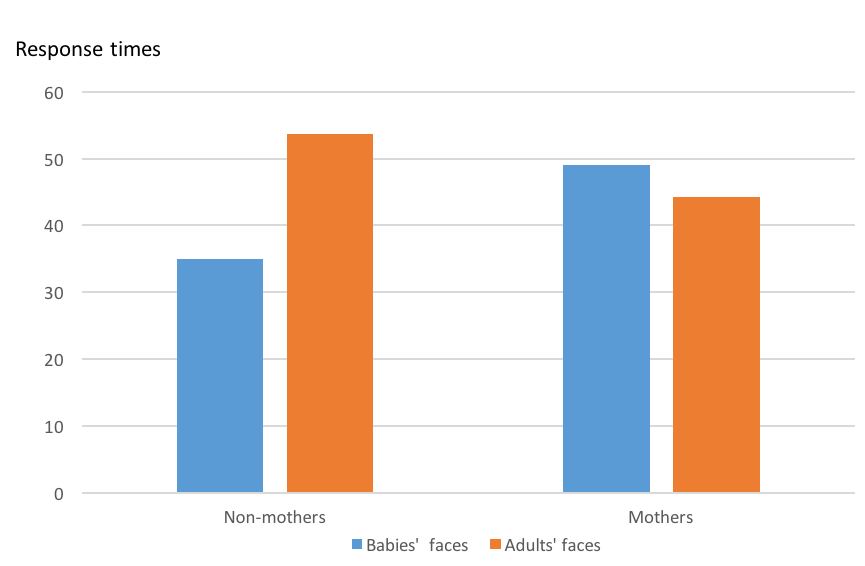
\includegraphics[width=\linewidth]{pictures/RT_identity_motherhood.png}
%     \centering
%     \caption{Stroop effect of response times}
%   \end{subfigure}
%   \begin{subfigure}[b]{0.4\linewidth}
%     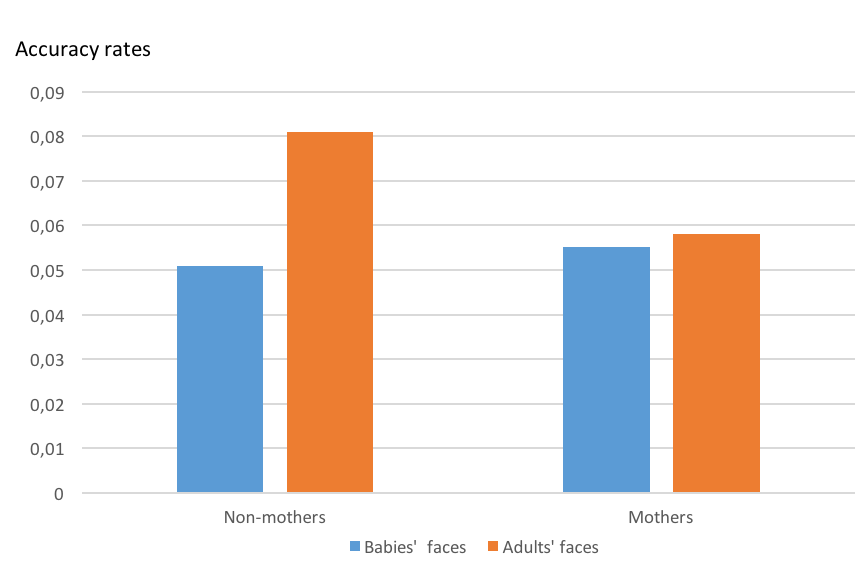
\includegraphics[width=\linewidth]{pictures/ACC_identity_motherhood.png}
%     \centering
%     \caption{Stroop effect of accuracy rates}
%   \end{subfigure}
%   \caption{The Stroop effects between different conditions of the sources of the facial expressions and status of the motherhood}
%   \label{fig.results.h3}
% \end{figure}

% \section{Additional effects}\label{sec.results.additional}
% As no significant difference in Stroop effect is found between when babies' faces are displayed and when adults' faces are displayed in the group of mothers, we intend to investigate whether the emotions of the facial expressions of the interference also has an influence over the effect. Therefore, we conduct two paired-samples t-tests. Significant results are found in the accuracy rates. 

\begin{figure}[!t]
  \centering
  \begin{subfigure}[b]{0.9\linewidth}
    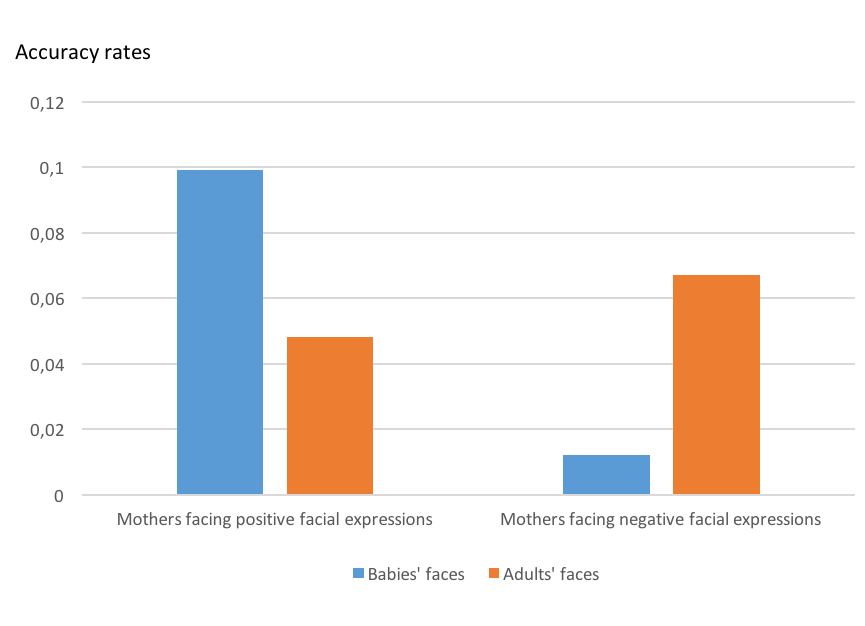
\includegraphics[width=\linewidth]{pictures/ACC_facialexp_identity.png}
    \caption{in the group of mothers}
  \end{subfigure}
  \begin{subfigure}[b]{0.9\linewidth}
    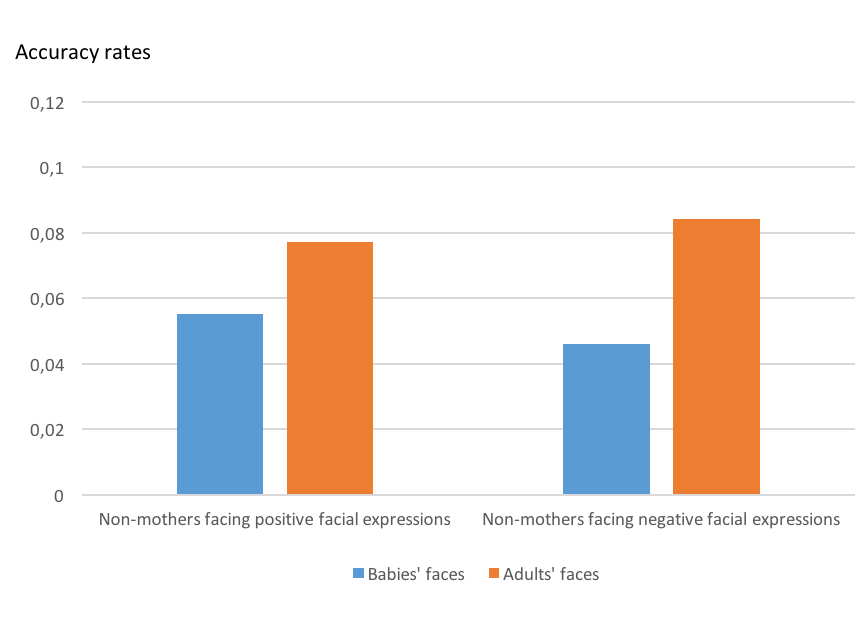
\includegraphics[width=\linewidth]{pictures/ACC_Nonmother_identity_facialexp.png}
    \caption{in the group of non-mothers}
  \end{subfigure}
  \caption{Stroop effect of the accuracy rates in the group of mothers as well as in the group of non-mothers when different sources and emotions of the facial expressions of the interference are presented}
  \label{fig.results.add}
\end{figure}





